%% Requires compilation with XeLaTeX or LuaLaTeX
\documentclass[aspectratio=169,10pt,xcolor={table,dvipsnames},t]{beamer}
\usetheme{UCBerkeley}
\hypersetup{colorlinks=true, linkcolor=blue, citecolor=blue, urlcolor=blue}
\usepackage{xcolor}

\title[lecture 05]{Next Generation Data Centers and Energy Management Systems}
\subtitle{Lecture 5B: Liquid Cooling \& Advanced Heat Transfer}
% Radiation heat transfer for Lecture 5c??? Data center cooling in space? 
\author{Prof. Thomas M. Schutzius}
\institute{Department of Mechanical Engineering}
\date{Fall 2026}

\begin{document}

\begin{frame}
  \titlepage
\end{frame}

% Uncomment these lines for an automatically generated outline.
%\begin{frame}{Outline}
%  \tableofcontents
%\end{frame}

\smallframetitle

{
\setbeamertemplate{background}{} % Hides background for this frame
\setbeamertemplate{footline}{}   % Reclaims the bottom space
	\begin{frame}
		\frametitle{Learning Plan}
%		% Commands to include a figure:
		\begin{itemize}
			\item Introduction to Data Center Systems and Thermodynamics 
			\item Psychrometrics and Heat Transfer
			\item Performance Metrics and Standards
			\item Applied Computational Fluid Dynamics (CFD)
			\item \textbf{Liquid Cooling \& Advanced Heat Transfer}
			\item Chip Cooling: Heat Conduction and Thermal Interface Materials 
			\item Power Delivery and Infrastructure (Energy sources: Geothermal, Solar, Nuclear, etc.)
			\item Overview of Simulation Field; the Concept of a Digital Twin 
			\item Machine Learning and Optimization Tools 
			\item Modeling and Simulation of an Energy Management System 
			\item Control Systems and Optimization 
			\item Spacecraft Thermal Control
			\item Final Project Work, Peer Feedback, and Mentor Check-in 
			\item Symposium 
		\end{itemize}		
	\end{frame}
}


% \setbeamertemplate{background}{} % Hides background for this frame
% \setbeamertemplate{footline}{}   % Reclaims the bottom space


	\begin{frame}
		\frametitle{Learning Objectives}
%		% Commands to include a figure:
		\begin{itemize}
			\item Explain the physical limitations of air cooling in high-thermal design power environments.
			\item Identify the key components used to transfer heat away from a chip (TIMs, spreaders, heat pipes).
			\item Differentiate between various liquid cooling architectures (Cold Plates vs. Immersion).
			\item Describe the role and function of a cooling distribution unit (CDU) in a data center environment.
		\end{itemize}		
	\end{frame}

\begin{frame}
	\frametitle{Seminar 2}
		\begin{itemize}
			\item Dr. David Geb, Synopsys (formerly Ansys)
			\item Title: TBD
			\item Date: Tuesday, 9/29/26
			\item Time: 15:30 (Berkeley Time)
			\item Location: GSPP 150
		\end{itemize}
\end{frame}

{
\setbeamertemplate{background}{} % Hides background for this frame
\setbeamertemplate{footline}{}   % Reclaims the bottom space
\smallframetitle
\begin{frame}
	\frametitle{Typical layout of a data center facility}
		\begin{figure}
			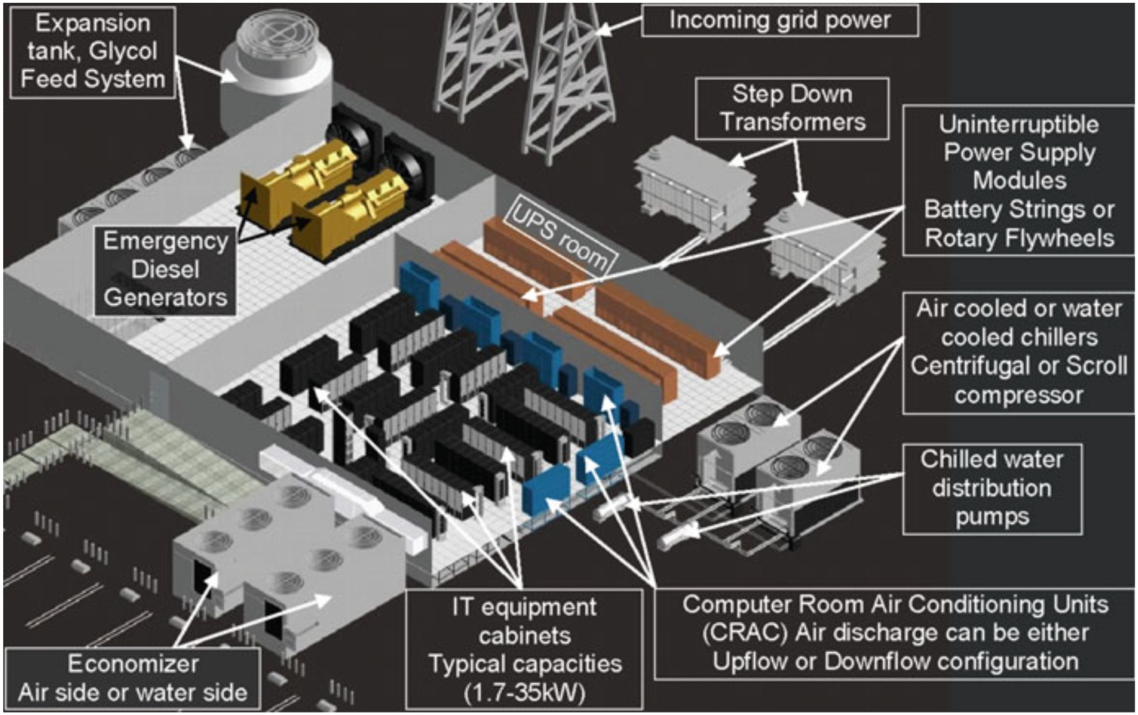
\includegraphics[width=0.65\textwidth]{../figures/joshi2021introduction-figure-01-01.pdf}
%			\vspace{-0.5cm}
		 \caption{(Figure 1.1 in Ref. \cite{joshi2012energy}).}
		\end{figure}
\end{frame}
}

	\begin{frame}{Liquid cooling}
		\begin{itemize}
			\item \textbf{Power Density:} Increasing TDP (thermal design power) leads to extreme heat fluxes at the chip level.
			\item \textbf{Limitations of Air:}
			\begin{itemize}
				\item Low volumetric heat capacity.
				\item Requires large volumes of air and high fan speeds (power intensive).
				\item Limited heat transfer coefficient.
			\end{itemize}
			\item \textbf{The Liquid Advantage:}
			\begin{itemize}
				\item Much higher thermal conductivity and heat capacity.
				\item Allows for much higher heat flux removal in a smaller footprint.
			\end{itemize}
		\end{itemize}
	\end{frame}



{
\setbeamertemplate{background}{} % Hides background for this frame
\setbeamertemplate{footline}{}   % Reclaims the bottom space
\smallframetitle
\begin{frame}
	\frametitle{\href{https://datahub.berkeley.edu/user-redirect/git-pull?repo=https://github.com/mtsn-lab/me137-237a&subPath=examples/fanLaws.ipynb}{Fan Laws}}

% This derivation comes from Ref.\cite{bejan2004convection}.
		\begin{figure}
			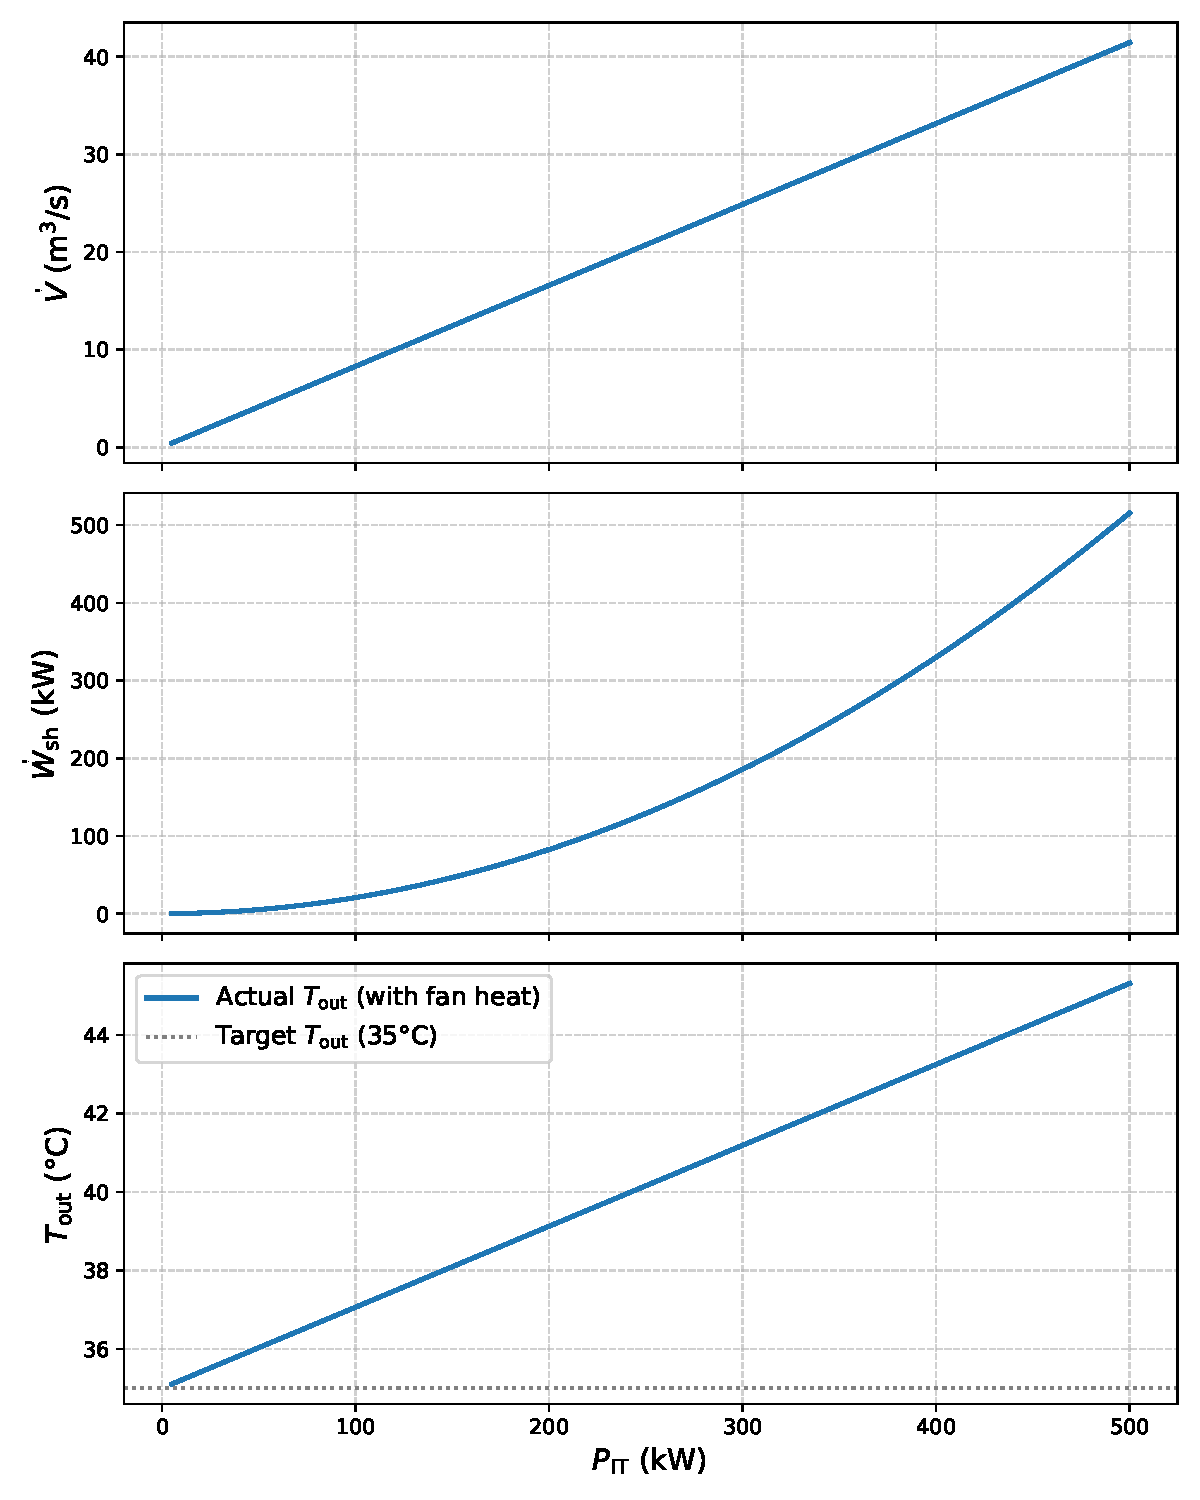
\includegraphics[width=0.4\textwidth]{../figures/rack_cooling_plots.pdf}
%			\vspace{-0.5cm}
%		 \caption{Solution to the Pohlhausen equation. Read his biography \href{https://doi.org/10.1146/annurev.fl.16.010184.000245}{here}.}
		\end{figure}
\end{frame}
}

	\begin{frame}{Cooling technologies}
		\begin{figure}
			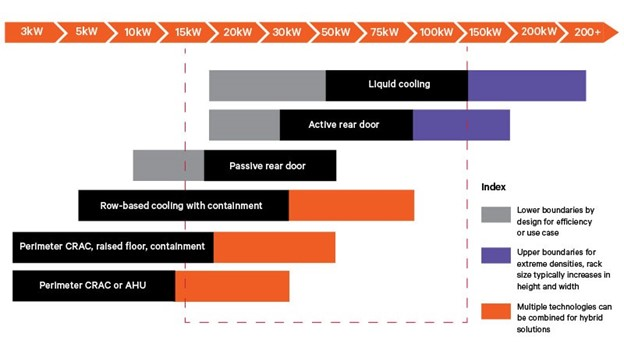
\includegraphics[width=0.5\textwidth]{../figures/800x450-figure-1-cooling-technology.jpg}
%			\vspace{-0.5cm}
		 \caption{Understanding direct-to-chip cooling in HPC infrastructure: A deep dive into liquid cooling. Ref: \href{https://www.vertiv.com/en-us/insights/articles/educational-articles/understanding-direct-to-chip-cooling-in-hpc-infrastructure-a-deep-dive-into-liquid-cooling/}{Vertiv}.}
		\end{figure}
	\end{frame}


	\begin{frame}{Thermal Interface Materials (TIM)}
		\begin{itemize}
			\item \textbf{The Problem:} Surface roughness at the chip/spreader interface creates microscopic air gaps (insulators).
			\item \textbf{The Solution:} TIMs (greases, pads, liquid metal) fill these gaps to create a continuous conduction path.
			\item \textbf{Key Metrics:}
			\begin{itemize}
				\item \textbf{Thermal Conductivity ($k$):} Higher is better.
				\item \textbf{Bond line thickness:} Minimizing thickness reduces total thermal resistance ($R_{th}$).
			\end{itemize}
		\end{itemize}
	\end{frame}

	\begin{frame}{Heat Spreaders}
		\begin{itemize}
				\item High-conductivity metal (usually copper) to distribute heat laterally.
				\item Reduces "spreading resistance."
		\end{itemize}
	\end{frame}
	
	
	\begin{frame}{Heat pipes and vapor chambers}
			\begin{itemize}
				\item Use phase change (evaporation/condensation) to transport heat.
				\item Heat pipe: 1D transport via capillary action.
				\item Vapor chamber: 2D spreading via phase change; extremely efficient for high-flux chips.
			\end{itemize}
			
  \begin{columns}
    \begin{column}{0.3\textwidth}
		\begin{figure}
			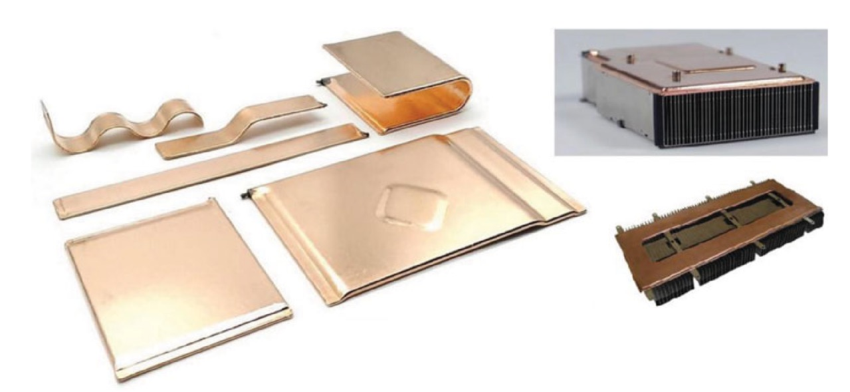
\includegraphics[width=1\textwidth]{../figures/bulut2019review-fig-1.pdf}
%			\vspace{-0.5cm}
		 \caption{Various vapor chambers \cite{bulut2019review}.}
		\end{figure}
    \end{column}
    
    \begin{column}{0.3\textwidth}
		\begin{figure}
			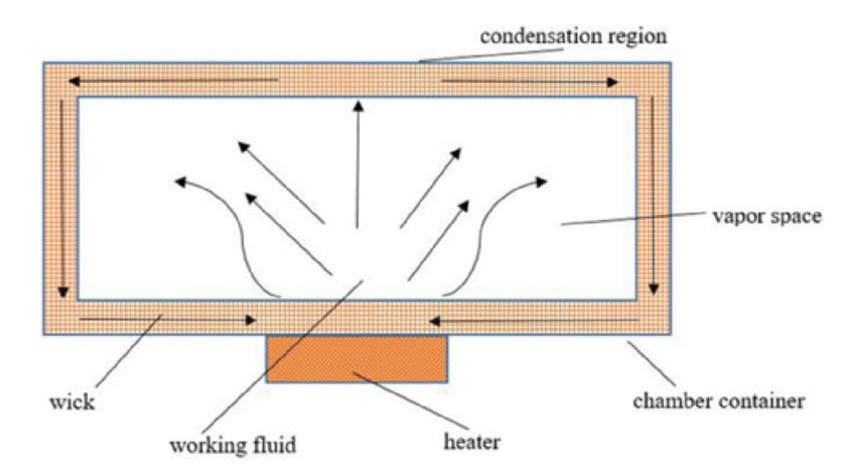
\includegraphics[width=1\textwidth]{../figures/bulut2019review-fig-2.pdf}
%			\vspace{-0.5cm}
		 \caption{Structure of a vapor chamber (Schematic: dimensions and sizes are not to scale) \cite{bulut2019review}.}
		\end{figure}
    \end{column}
  \end{columns}
	\end{frame}
	
	\begin{frame}{\href{https://datahub.berkeley.edu/user-redirect/git-pull?repo=https://github.com/mtsn-lab/me137-237a&subPath=examples/heatPipesVaporChambers.ipynb}{Heat pipes and vapor chambers}}
		\begin{figure}
			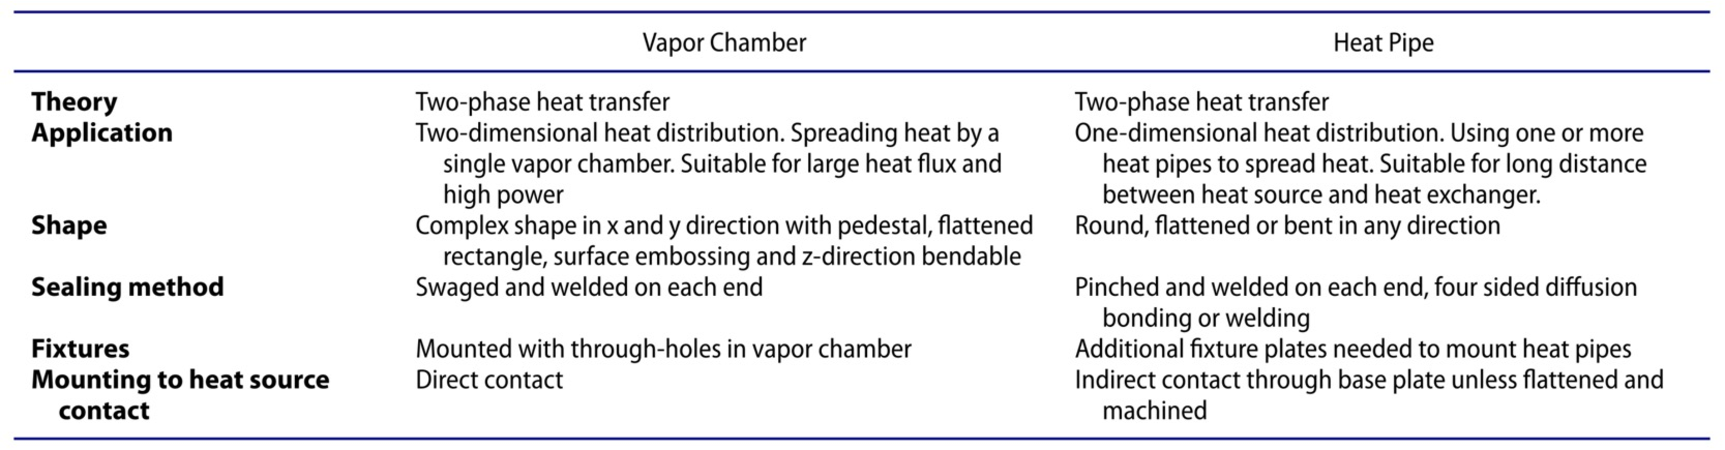
\includegraphics[width=0.8\textwidth]{../figures/bulut2019review-tab-1.pdf}
%			\vspace{-0.5cm}
		 \caption{A comparison between vapor chambers and heat pipes \cite{bulut2019review}. See also Ref.\cite{jouhara2023heat}.}
		\end{figure}
	\end{frame}


	

	\begin{frame}{Liquid Cooling Architectures: Cold Plates}
		\begin{itemize}
			\item \textbf{Direct-to-Chip (cold plate) Cooling:}
			\begin{itemize}
				\item A liquid-cooled metal block is mounted directly to the chip.
				\item Liquid flows through internal channels to absorb heat.
				\item \href{https://www.youtube.com/watch?v=98xtaYz0sy8}{Video} of the ``skiving'' process.
			\end{itemize}
			\item \textbf{Microchannel Technology:}
			\begin{itemize}
				\item Etching tiny channels into the cold plate to vastly increase the surface area.
				\item Maximizes the convective heat transfer coefficient ($h$).
			\end{itemize}
		\end{itemize}
	\end{frame}

	\begin{frame}{Liquid Cooling Architectures: Immersion}
		\begin{itemize}
			\item \textbf{The Concept:} Submerging the entire IT hardware in a dielectric (non-conductive) fluid.
			\item \textbf{Single-Phase Immersion:}
			\begin{itemize}
				\item Fluid remains liquid; cooled via convection and circulated by pumps.
			\end{itemize}
			\item \textbf{Two-Phase Immersion:}
			\begin{itemize}
				\item Fluid boils at the chip surface.
				\item Utilizes \textbf{latent heat of vaporization} for superior cooling.
			\end{itemize}
		\end{itemize}
	\end{frame}
	
	\begin{frame}{System-Level: Cooling Distribution Unit (CDU)}
		\begin{itemize}
			\item \textbf{The Role:} Manages the heat exchange between the facility water and the IT cooling loop.
			\item \textbf{Two-Loop System:}
			\begin{itemize}
				\item \textbf{Primary Loop:} Facility water (chilled water from the building).
				\item \textbf{Secondary Loop (TCS):} Treated/dielectric fluid that circulates through the servers.
			\end{itemize}
			\item \textbf{Core Functions:}
			\begin{itemize}
				\item Heat Exchange (Plate Heat Exchangers).
				\item Pumping and Flow Control.
				\item Filtration and Water Chemistry Management.
				\item Leak Detection and Safety Monitoring.
			\end{itemize}
		\end{itemize}
	\end{frame}
	
	\begin{frame}{System-Level: Cooling Distribution Unit (CDU)}
		\begin{figure}
			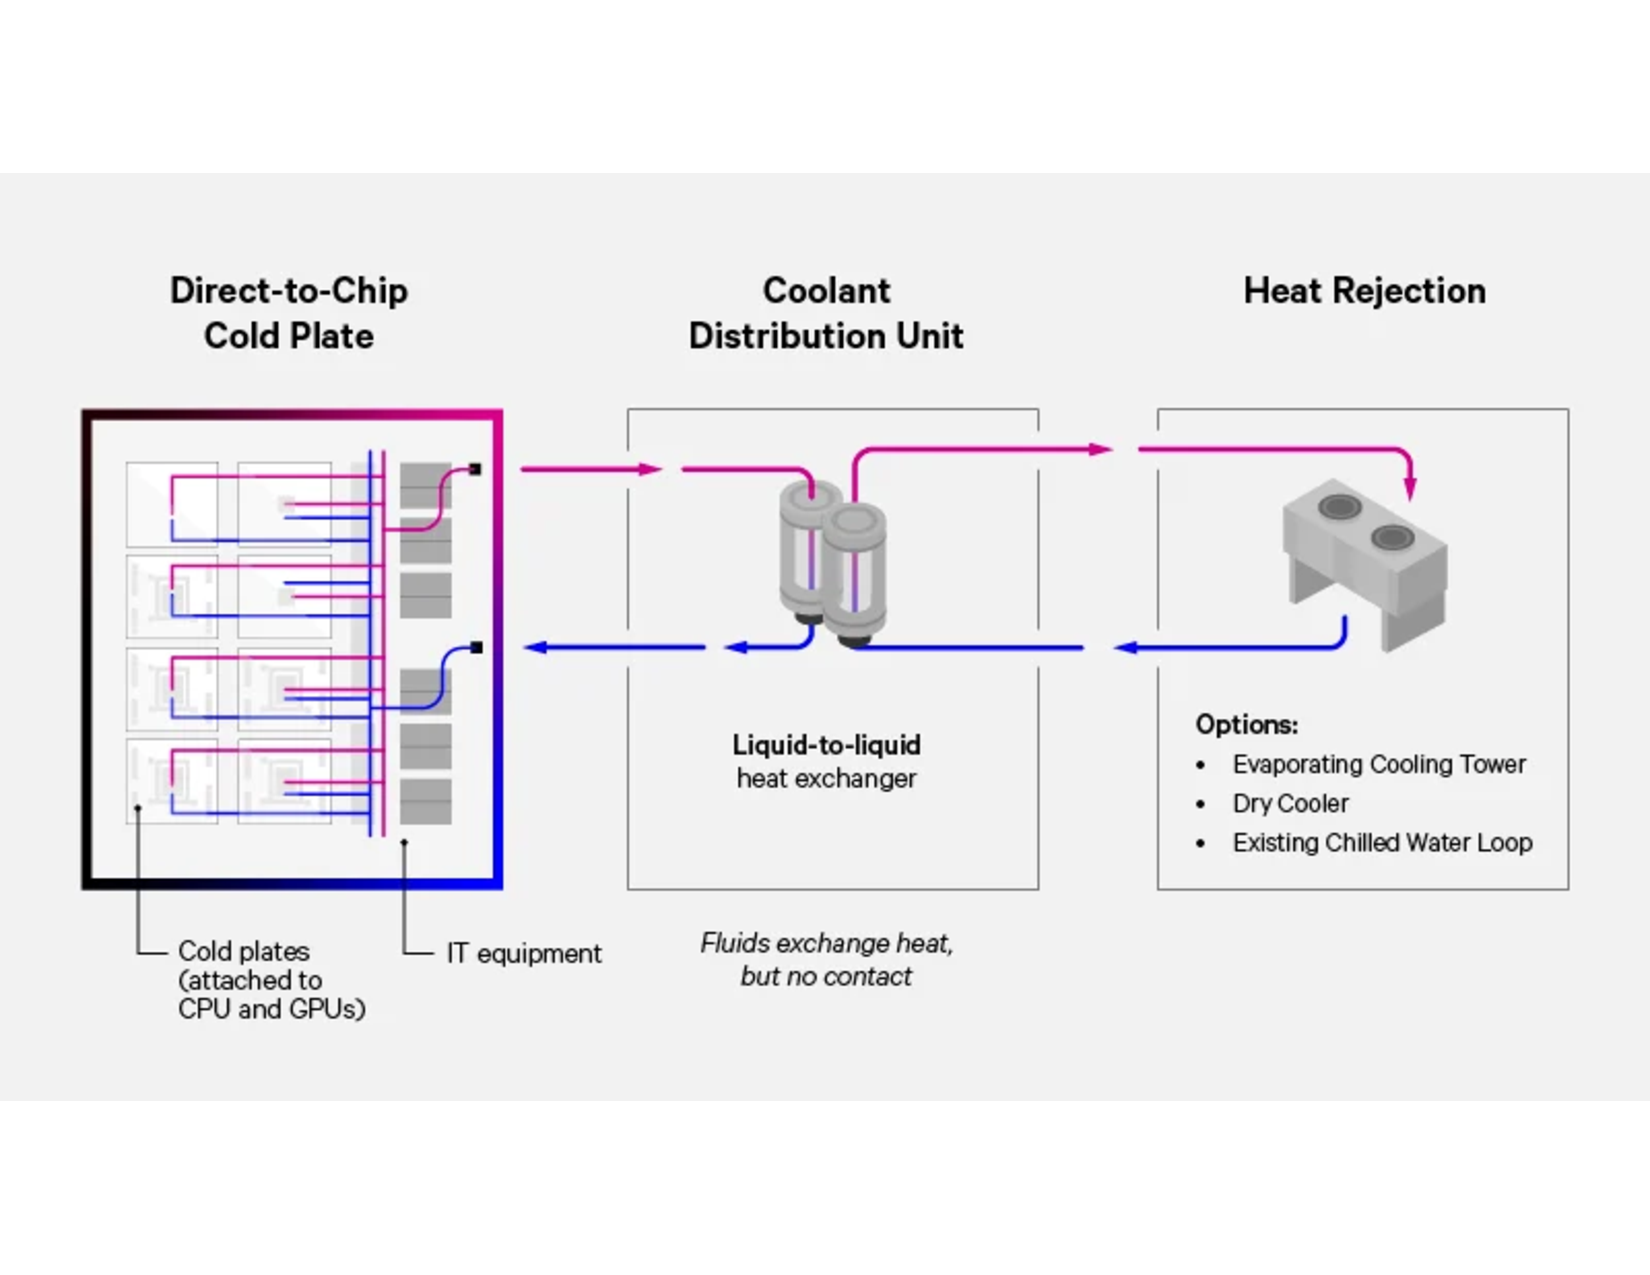
\includegraphics[width=0.5\textwidth]{../figures/vertiv-direct-to-chip-cold-plate.pdf}
			\vspace{-0.5cm}
		 \caption{\href{https://www.vertiv.com/en-us/solutions/vertiv-high-density-cooling-solutions/}{Vertiv}.}
		\end{figure}
	\end{frame}

	\begin{frame}{Case Study: Aquasar Technology}
		\begin{itemize}
			\item \textbf{Concept:} A hot water cooled supercomputer prototype designed for direct energy reuse \cite{zimmermann2012aquasar}.
			\item \textbf{Performance Comparison:}
			\begin{itemize}
				\item \textbf{Liquid (Hot Water):} $\Delta T_{chip/coolant} \approx 15^\circ\text{C}$ (at $60^\circ\text{C}$ coolant).
				\item \textbf{Air Cooling:} $\Delta T_{chip/air} \approx 35^\circ\text{C}$ (requiring pre-cooling to $23^\circ\text{C}$).
			\end{itemize}
			\item \textbf{Key Advantages:}
			\begin{itemize}
				\item Eliminates the need for energy-intensive chillers.
				\item Enables \textbf{Heat Reuse}: $60^\circ\text{C}$ water can be used for building heating.
				\item \textbf{Efficiency:} Achieved 80\% heat recovery efficiency and 34\% exergetic efficiency.
			\end{itemize}
			\item \textbf{Economic Insight:} Space heating provides the highest economic value for recovered heat.
		\end{itemize}
	\end{frame}	
	
	\begin{frame}{\href{https://datahub.berkeley.edu/user-redirect/git-pull?repo=https://github.com/mtsn-lab/me137-237a&subPath=examples/fanLaws.ipynb}{Case Study: Aquasar Technology}}
		\begin{figure}
			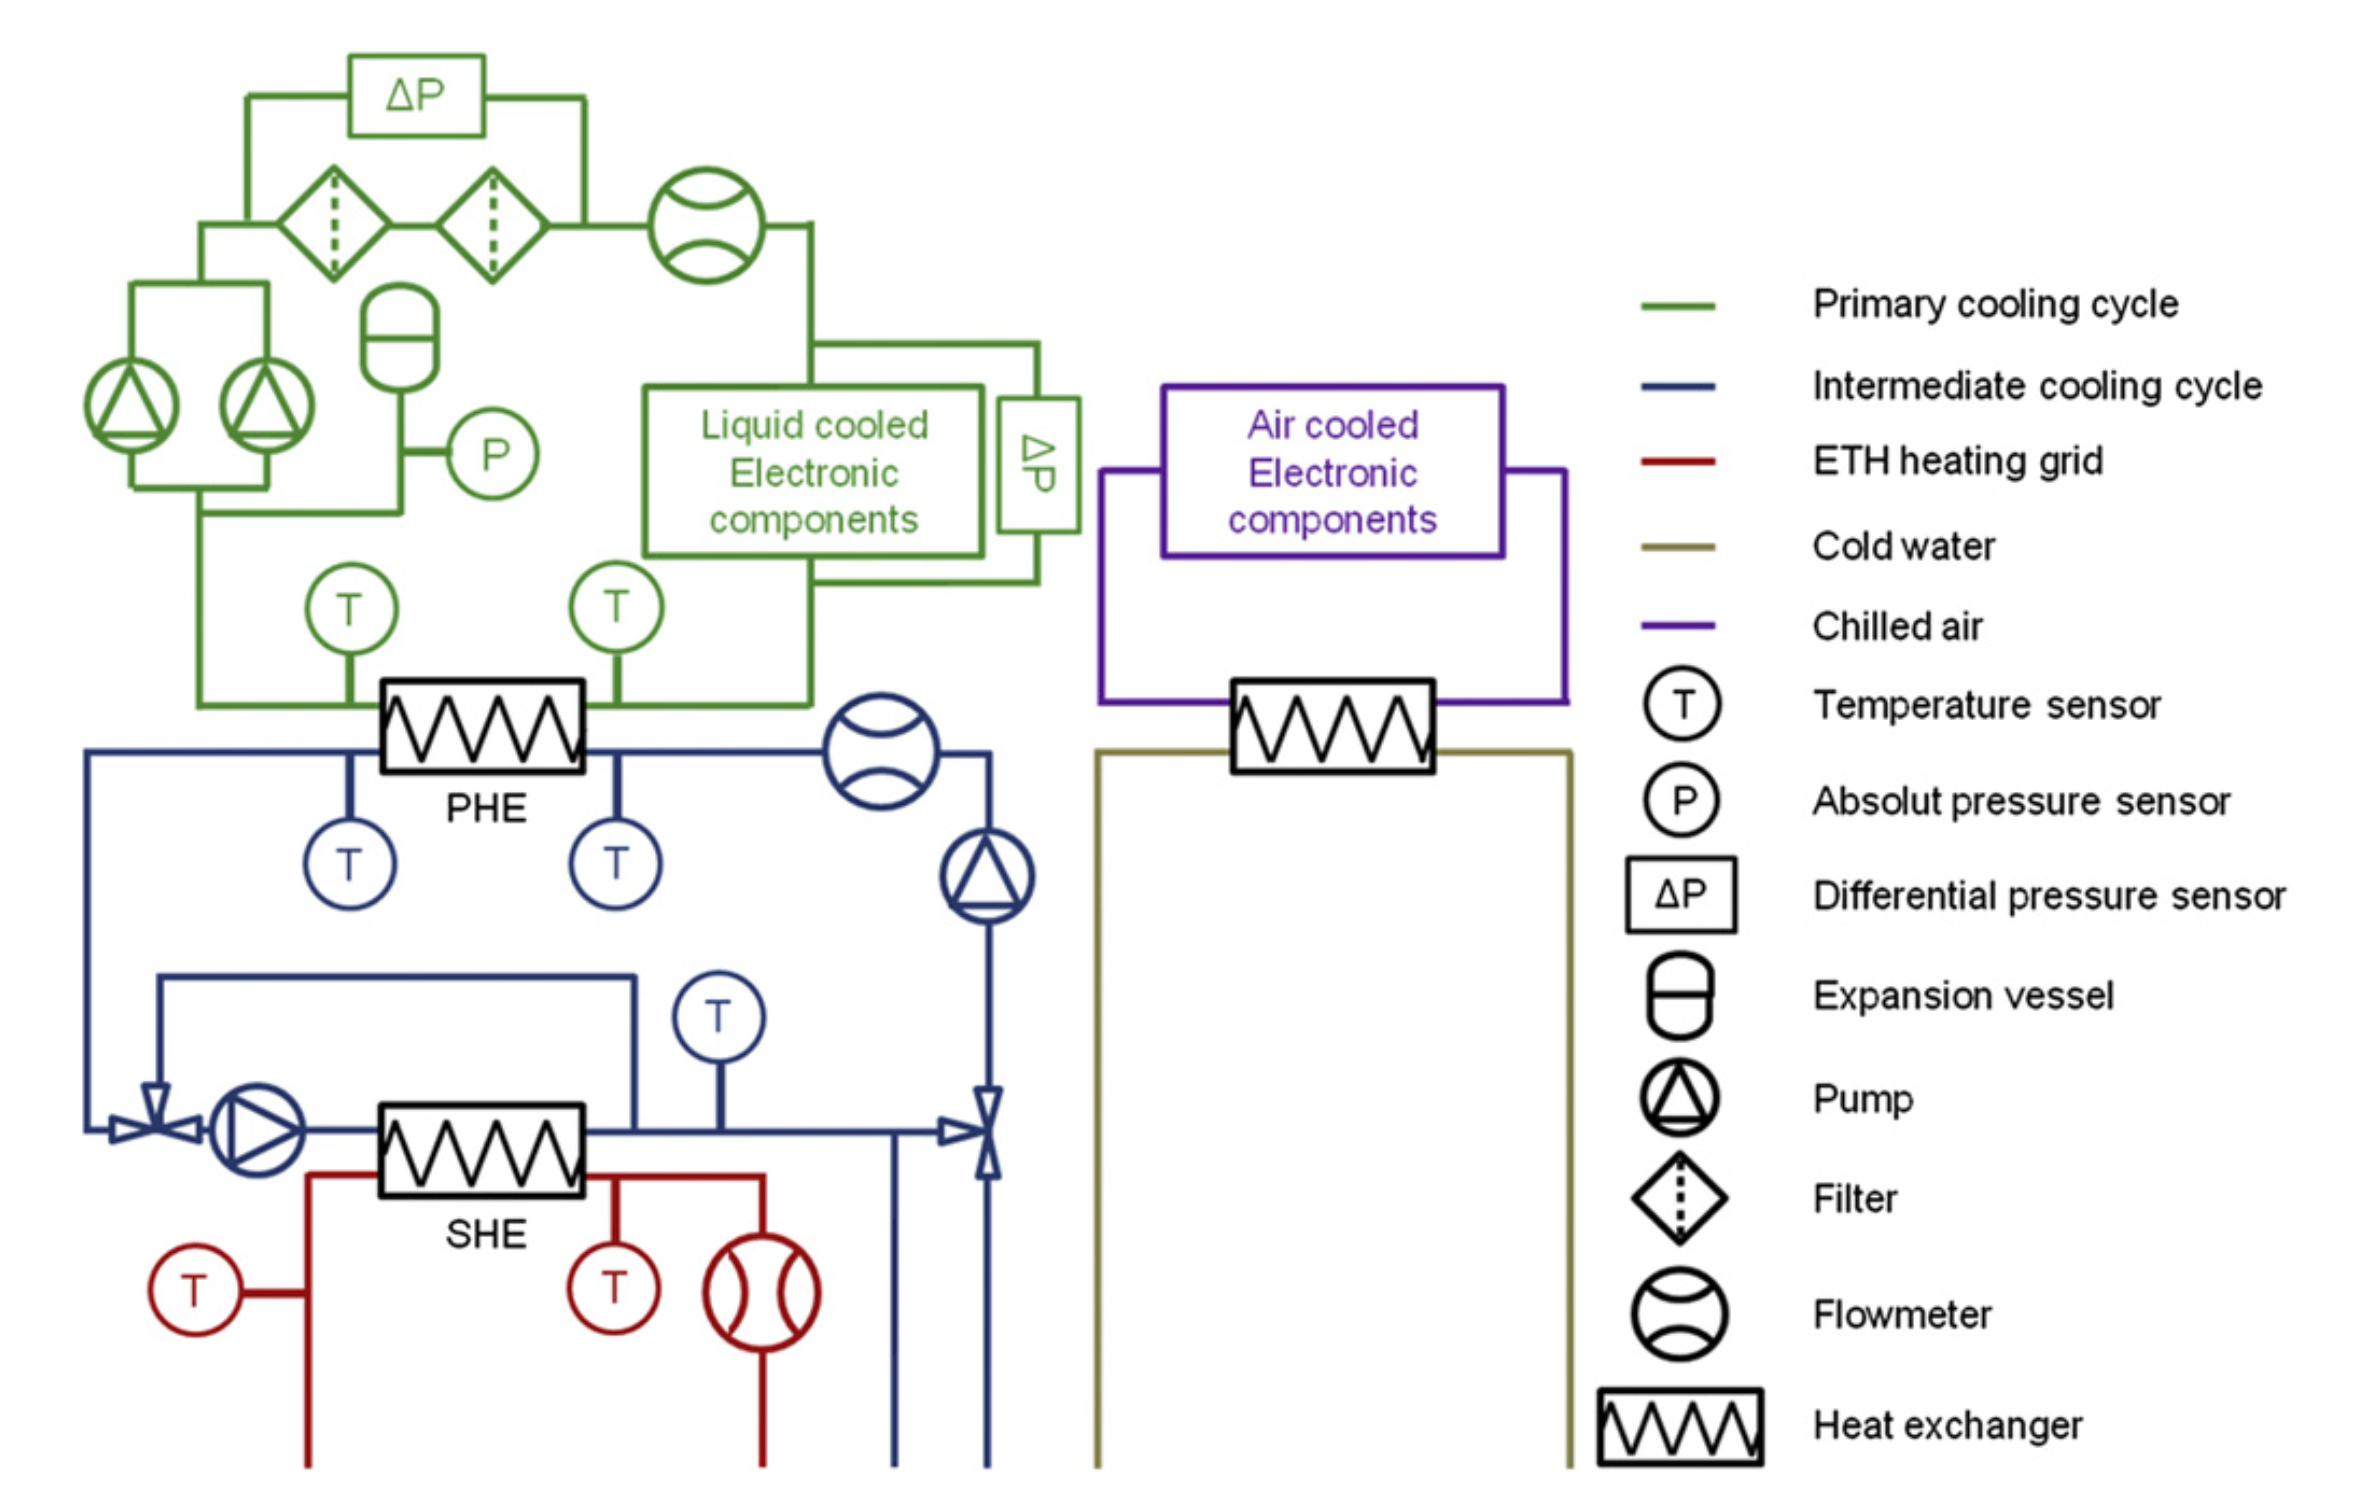
\includegraphics[width=0.5\textwidth]{../figures/zimmermann2012aquasar-fig-2.png}
%			\vspace{-0.5cm}
		 \caption{Aquasar: Schematics of the cooling loop \cite{zimmermann2012aquasar}. Let us analyze the second law efficiency of the green loop.}
		\end{figure}
	\end{frame}

	\begin{frame}{\href{https://datahub.berkeley.edu/user-redirect/git-pull?repo=https://github.com/mtsn-lab/me137-237a&subPath=examples/fanLaws.ipynb}{Case Study: Aquasar Technology}}
		\begin{figure}
			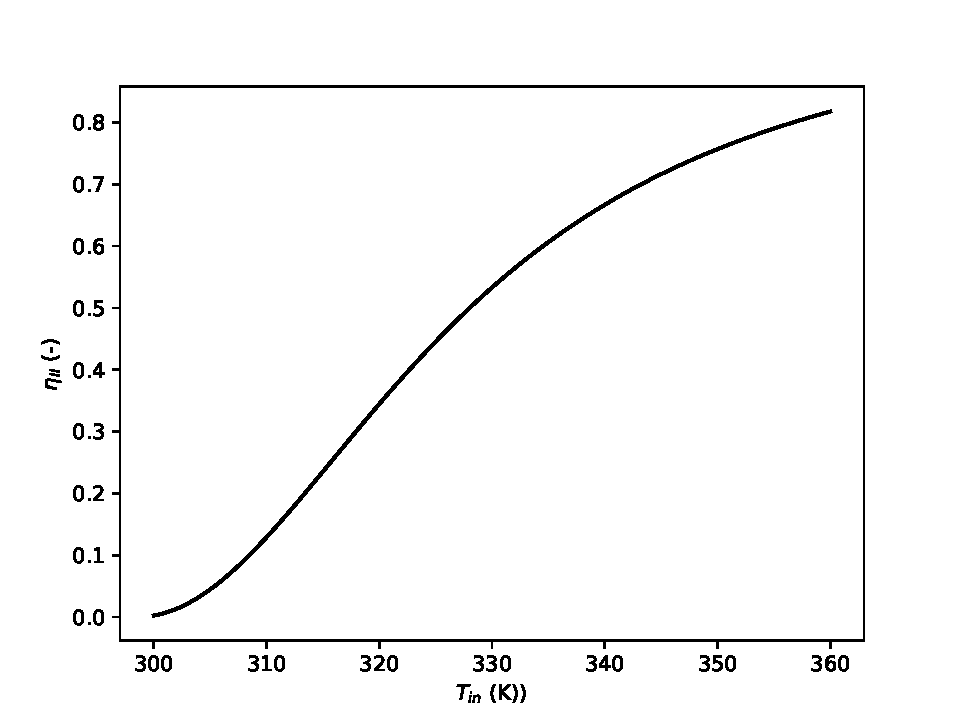
\includegraphics[width=0.5\textwidth]{../figures/eta-Tin.pdf}
			\vspace{-0.5cm}
		 \caption{Second-law efficiency of the secondary TCS loop  \cite{zimmermann2012aquasar}.}
		\end{figure}
	\end{frame}



	\begin{frame}{Radiative Cooling in Space Systems}
		\begin{itemize}
			\item \textbf{The Challenge:} In the vacuum of space, there is no atmosphere for convection or conduction to a medium. \textbf{Radiation} is the only mechanism for heat rejection.
			\item \textbf{The Thermal Path:}
			\begin{itemize}
				\item High-power chips $\rightarrow$ Liquid/Pumped Loops $\rightarrow$ External Radiator Panels $\rightarrow$ Deep Space.
			\end{itemize}
			\item \textbf{Physics (Stefan-Boltzmann Law):}
			\begin{equation*}
				Q_{rad} = \epsilon \sigma A (T_{rad}^4 - T_{space}^4)
			\end{equation*}
			\item \textbf{Key Design Considerations:}
			\begin{itemize}
				\item \textbf{High Emissivity ($\epsilon$):} Using specialized coatings to maximize heat rejection.
				\item \textbf{Radiator Area ($A$):} Large surface areas are required due to the $T^4$ dependence.
				\item \textbf{Solar/Albedo Loading:} Managing heat from the Sun or Earth that hits the radiator.
				\item \textbf{Mass Constraints:} Every kg of radiator/fluid adds to launch cost.
			\end{itemize}
		\end{itemize}
	\end{frame}

{
\setbeamertemplate{background}{} % Hides background for this frame
\setbeamertemplate{footline}{}   % Reclaims the bottom space
\setbeamertemplate{bibliography item}[text] % Replaces default icons with numbers
\smallframetitle
	\begin{frame}[allowframebreaks]{References}
		\bibliographystyle{plain}
		\bibliography{../../bibliography}
	\end{frame}
}

\end{document}
